%%%%%%%%%%%%%%%%%%%%%%%%%%%%%%%%%%%%%%%%%
% Short Sectioned Assignment
% LaTeX Template
% Version 1.0 (5/5/12)
%
% This template has been downloaded from:
% http://www.LaTeXTemplates.com
%
% Original author:
% Frits Wenneker (http://www.howtotex.com)
%
% License:
% CC BY-NC-SA 3.0 (http://creativecommons.org/licenses/by-nc-sa/3.0/)
%
%%%%%%%%%%%%%%%%%%%%%%%%%%%%%%%%%%%%%%%%%

%----------------------------------------------------------------------------------------
%	PACKAGES AND OTHER DOCUMENT CONFIGURATIONS
%----------------------------------------------------------------------------------------

\documentclass[paper=a4, fontsize=12pt]{scrartcl} % A4 paper and 11pt font size

\usepackage[T1]{fontenc} % Use 8-bit encoding that has 256 glyphs
\usepackage{fourier} % Use the Adobe Utopia font for the document - comment this line to return to the LaTeX default
\usepackage[english]{babel} % English language/hyphenation
\usepackage{amsmath,amsfonts,amsthm} % Math packages
\usepackage{listings}
\usepackage{graphicx}

\usepackage{lipsum} % Used for inserting dummy 'Lorem ipsum' text into the template

\usepackage{sectsty} % Allows customizing section commands
\allsectionsfont{\centering \normalfont\scshape} % Make all sections centered, the default font and small caps

\usepackage{fancyhdr} % Custom headers and footers
\pagestyle{fancyplain} % Makes all pages in the document conform to the custom headers and footers
\fancyhead{} % No page header - if you want one, create it in the same way as the footers below
\fancyfoot[L]{} % Empty left footer
\fancyfoot[C]{} % Empty center footer
\fancyfoot[R]{\thepage} % Page numbering for right footer
\renewcommand{\headrulewidth}{0pt} % Remove header underlines
\renewcommand{\footrulewidth}{0pt} % Remove footer underlines
\setlength{\headheight}{13.6pt} % Customize the height of the header

\numberwithin{equation}{section} % Number equations within sections (i.e. 1.1, 1.2, 2.1, 2.2 instead of 1, 2, 3, 4)
\numberwithin{figure}{section} % Number figures within sections (i.e. 1.1, 1.2, 2.1, 2.2 instead of 1, 2, 3, 4)
\numberwithin{table}{section} % Number tables within sections (i.e. 1.1, 1.2, 2.1, 2.2 instead of 1, 2, 3, 4)

\setlength{\parskip}{8pt}%
\setlength\parindent{0pt} % Removes all indentation from paragraphs - comment this line for an assignment with lots of text

%----------------------------------------------------------------------------------------
%	TITLE SECTION
%----------------------------------------------------------------------------------------

\newcommand{\horrule}[1]{\rule{\linewidth}{#1}} % Create horizontal rule command with 1 argument of height

\title{	
\normalfont \small 
\textsc{Penn State University, Department of Electrical Engineering \& Computer Science}
\horrule{0.5pt} \\[0.4cm] % Thin top horizontal rule
	\huge CMPEN 431 - Final Project \\ % The assignment title
\horrule{2pt} \\[0.5cm] % Thick bottom horizontal rule
}

% Author and Date
\author{Quang Nguyen \& Richard Heidorn}
\date{\normalsize \today}

% Homework
\begin{document}

\maketitle % Print the title

%----------------------------------------------------------------------------------------

Best IPC and Execution Time for \textbf{mcf} and \textbf{milc}:

\begin{center}
\begin{tabular}{ |c|c|c| } 
	\hline
	 & IPC & Execution Time \\ \hline
	Base mcf & & \\ \hline
	Base milc & & \\ \hline
	Best mcf & & \\ \hline
	Best milc & & \\ \hline
\end{tabular}
\end{center}

Best execution time \textbf{mcf} issue width and data path type: \\

Best execution time \textbf{milc} issue width and data path type: \\

Overall Best Execution Time Geometric Means:

\begin{center}
\begin{tabular}{ |c|c|c| } 
	\hline
	 & Geometric Mean \\ \hline
	Best Integer GM & \\ \hline
	Best Floating Point GM & \\ \hline
\end{tabular}
\end{center}

Best execution time GM Integer issue width and data path type: \\

Best execution time GM Floating Point issue width and data path type: \\


% Force the above to appear all on one page - the cover page. Start fresh for the content of the paper.
\newpage


\section{Introduction}

Designing a computer architecture is far from an exact science. A computer's performance is determined by many variables, ranging from the design and efficiency of the processor to the operating system and programs that run on top of the hardware. To name only a few, a computer's performance is determined by the functional units its processor contains, the length of its busses, the size and number of transistors, the organization of its caches, the speed and reliability of its hard drive, and ultimately the efficiency of its software.

By and large, computer architectures have become exponentially faster, smaller, more efficient, more durable, and more powerful. However, the number of factors that predict the performance of programs with the hardware is so great, it is nearly impossible to predict the most efficient computer designs for any given purpose. After all, the design that is optimal for one application might be sluggish for another. Even the same program, given a different set of data to compute, could perform better on different architectures.

For this project, we've investigated many different computer architectures using the Simple Scalar architecture simulator and how they affect the overall geometric means for four integer benchmarks and two floating point benchmarks provided by the SPEC performance benchmark package. The four integer benchmarks - bzip2, hmmer, mcf, sjeng - and two floating point benchmarks - milc, equake - were used to evaluate the overall performances of each tested architecture, and to evaluate how certain changes to the architectures would impact the programs' performance.


\subsection{Testing Methodology}

Simple Scalar provides a number of parameters that can be modified to emulate any modern computer architecture design. While the number and purpose of the parameters is easy to understand, the combinations of different parameters is incredibly large and difficult to comprehend. Thankfully, the project has been defined to limit the number of architectures that could be tested, but the sum total of all combinations is far greater than can be reasonably tested in a few weeks' time. Therefore, a brute force approach to determining the best design is impractical at best.

However, due to the number of variables outside of the architecture - the algorithms, access patterns, and behavior of the programs tested - it is not simply good enough to make educated guesses based on our understanding of processor evolution. Instead, a combination approach is required. Scientific reasoning is necessary to isolate the parameters and restrict the range of values which could benefit the performance of a given design. Once the parameters are defined and the range of reasonable values determined, a series of tests need to be run to experimentally verify our predictions and also to determine the best design decisions for a given architecture.

Our testing methods combine scientific analysis and experimental verification, both to determine which variables to test and which tests to run for all static and dynamic issue machines. Following each suite of tests, we identified and analyzed those designs which worked best for each machine and issue width. We've run dozens of test suites which isolated different components of the processor's functional units, branch prediction, instruction issuing, cache design, and the TLB. Each of these tests suites contained dozens to hundreds of individual configurations, all of which provided experimental information that were used to advance our designs to find a performant system. These tests were not comprehensive in any way, but we believe that we've isolated strong designs as a result of our methodology.

\subsection{Calculating the Geometric Mean}

The geometric means were calculated using the program execution times as its input. Since performance is typically defined as the inverse of the execution time, a smaller geometric mean translates to greater overall performance. The geometric mean is defined as:
\begin{align*}
	\text{Geometric Mean} &= \sqrt[n] {\prod_{i=1}^{n} \text{Execution Time}} \\
	&= \sqrt[n] {\prod_{i=1}^{n} \frac{\text{Instruction Count}_i \times \text{Clock Cycle}_i}{\text{Instructions Per Cycle}_i}} 
\end{align*}


\section{Order of Experimentation}

The majority of experiments were carried out by changing a few related parameters and determining how changing the variables affected the geometric means for all machine issue widths. By default, most of the tests were performed for both static and dynamic machines, with issue widths 1, 2 and 4 for static, and 2, 4, and 8 for dynamic. Near the end of our experimentation, we found that dynamic far outperformed static. To allow us to continue to test with higher accuracy, the static tests were eventually dropped in favor of the dynamic tests.

The order of our initial tests were mostly arbitrary and experimental, but we've found that there is a logical sequence for how testing could be performed. After reviewing our process, the ideal experimentation order would have been to isolate the independent variables that allow us to optimize the performance of all issue widths, to set these variables to their best performing values, and then to test the remaining inter-dependent variables. We present the order of experimentation as we've proceeded, but we focus on the experiments that yielded the most useful results.

\subsection{Identifying Independent Variables}

The first round of experimentation involved testing different, interrelated parameters, and determining how well they affected the geometric means independent of the other Simple Scalar parameters. For our tests, we began by first testing the ideal number of ALUs and Multipliers, Fetch Speed, Memory Width, and the Register Update Unit \& Load / Store Queue. The results for the ALU's / Multipliers and the Fetch Speed were mixed at best, and were ultimately inconclusive to test so early on. However, the results for the Memory Width and the Register Update Unit showed positive trends that we could use to build on.

\subsubsection{Best of the Register Update Unit \& Load / Store Queue}

For the register update unit (RUU) and load / store queue (LSQ), we found that the best performing designs for dynamic issue machines of 2-wide, 4-wide and 8-wide performed best when the number of RUUs or LSQs were maxed out for each issue width:
\begin{center}
\begin{tabular}{ |c|c|c| } 
	\hline
	Issue Width & RUU & LSQ  \\ \hline
	2-wide & 16 & 8 \\ \hline
	4-wide & 32 & 16 \\ \hline
	8-wide & 64 & 32 \\ \hline
\end{tabular}
\end{center}

These results stood across the board, which allowed us to progress with the remainder of our testing by optimizing the performance of all issue widths.

\subsubsection{Best of the Memory Width}

Seemingly a no-brainer now, the memory width needs to be maxed out at 16 for optimal performance. This value was tested against all 6 machine combinations.


\subsection{Branch Prediction: Finding an Ideal Method}

The branch predictors were tested heavily following the initial evaluation of the RUU, LSQ and memory width. We made the assumption that not-taken and taken will not perform as well as bimodal, two-level or the combination branch predictors, and this was verified after the original tests against the three best-performing branch predictors.

\subsubsection{Assumptions about the L1 Cache}

For the three tested branch predictors, we analyzed not only the performance of the different branch prediction methods, but we also performed extensive research into the L1 data and instruction caches and the unified L2 cache. In order for the branch prediction tests to be carried out in a timely manner, we made a decision to match the L1 instruction cache to the L1 data cache, while keeping them separated. While this may cause less-than-ideal combinations of both the data and instruction cache, the number of combinations was too great to reasonably analyze. Further, it is common to see instruction and data caches with matching specifications, which aided our decision to simplify the testing process.

While we realize that the more variables being tested, the more complex that the result analysis becomes, we were comfortable altering both the branch prediction type and altering the L1 and L2 caches. The same exact combinations of cache values were tested across all three branch predictors, which gave us a large number of results to compare the performance of each type of branch predictor. Ultimately, we saw that the combination method won out - not comfortably, but consistently enough that allowed us to expand our testing of the combination branch predictor. Of the hundreds of tests we ran, Figures \ref{fig:bpsi} through \ref{fig:bpdi} show the number of tests ran that returned a geometric mean at or below 1000 for both static and dynamic issue width systems. These figures also include expanded evaluation of the combination method, which is why the number of tests run for combination vastly exceeds bimodal and 2-level.

\begin{figure}
\centering
\begin{minipage}{0.5\textwidth}
\centering
	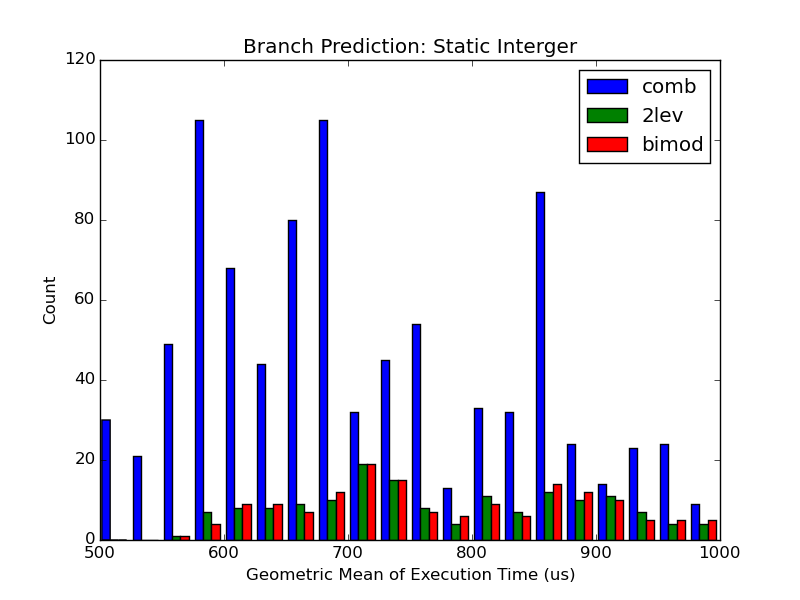
\includegraphics[width=\linewidth]{graphs/branch_prediction/Branch_Prediction_Static_Interger.png}
\end{minipage}\hfill
\begin{minipage}{0.5\textwidth}
\centering
 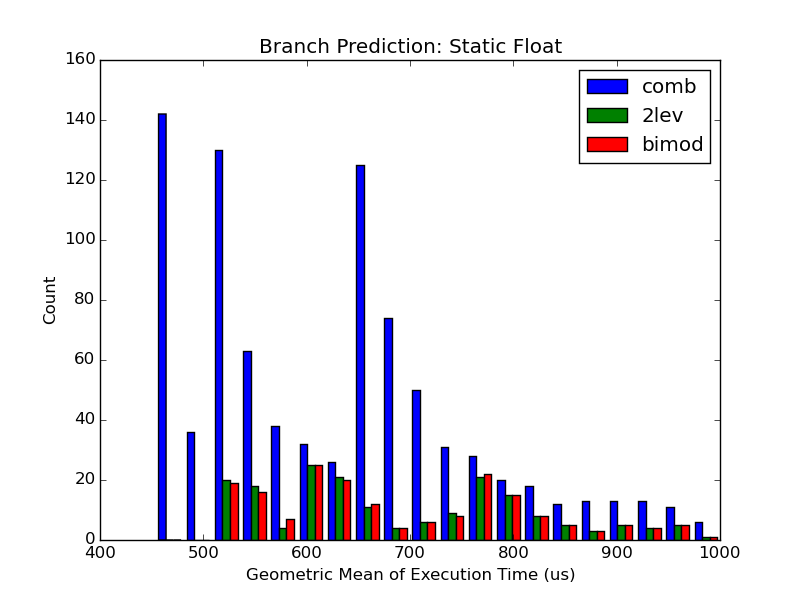
\includegraphics[width=\linewidth]{graphs/branch_prediction/Branch_Prediction_Static_Float.png}
\end{minipage}

\caption{A subset of the total tests run for three branch predictor types (bimodal, 2-level, combination) for static issue machines.}
\label{fig:bpsi}
\end{figure}

\begin{figure}
\centering
\begin{minipage}{0.5\textwidth}
\centering
	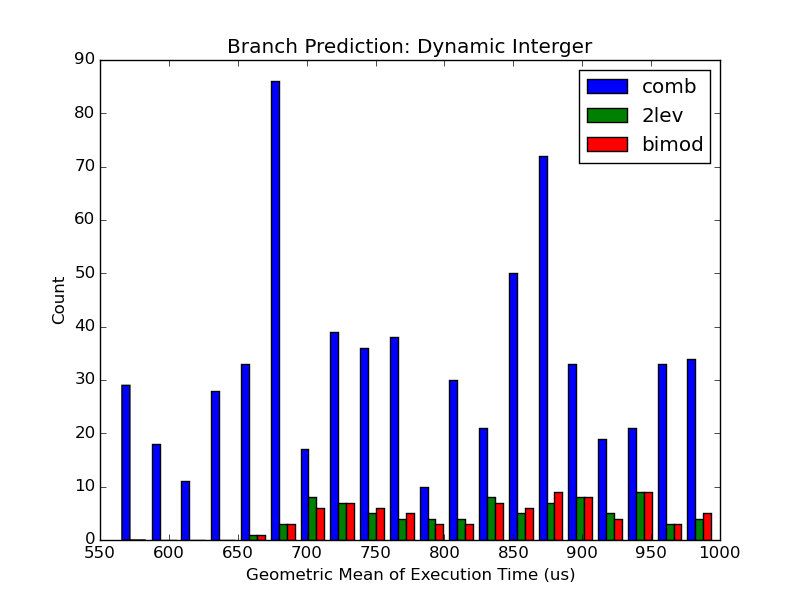
\includegraphics[width=\linewidth]{graphs/branch_prediction/Branch_Prediction_Dynamic_Interger.png}
\end{minipage}\hfill
\begin{minipage}{0.5\textwidth}
\centering
 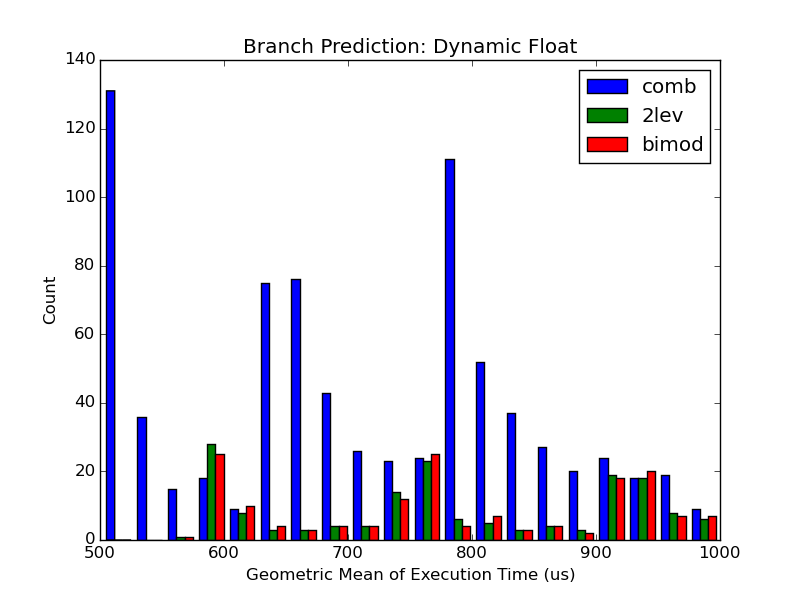
\includegraphics[width=\linewidth]{graphs/branch_prediction/Branch_Prediction_Dynamic_Float.png}
\end{minipage}

\caption{A subset of the total tests run for three branch predictor types (bimodal, 2-level, combination) for dynamic issue machines.}
\label{fig:bpdi}
\end{figure}


\subsection{TLB Investigation}

We expanded our search of independent variables by exploring the affect of various sizes of the TLB on the performance of the different machines. The results were not very surprising, as the use of the TLB is minimal compared to the time spent in the cache or performing operations. Ultimately, the effects of changing the different sizes of the associativity and the number of sets of the TLB had little impact on the final outcome of the geometric means for each of the machines. We've presented our findings for each machine and issue width in Figure \ref{fig:tlb}, for those machines / widths that managed a geometric mean below 1000.

\begin{figure}
\centering
\begin{minipage}{0.5\textwidth}
\centering
	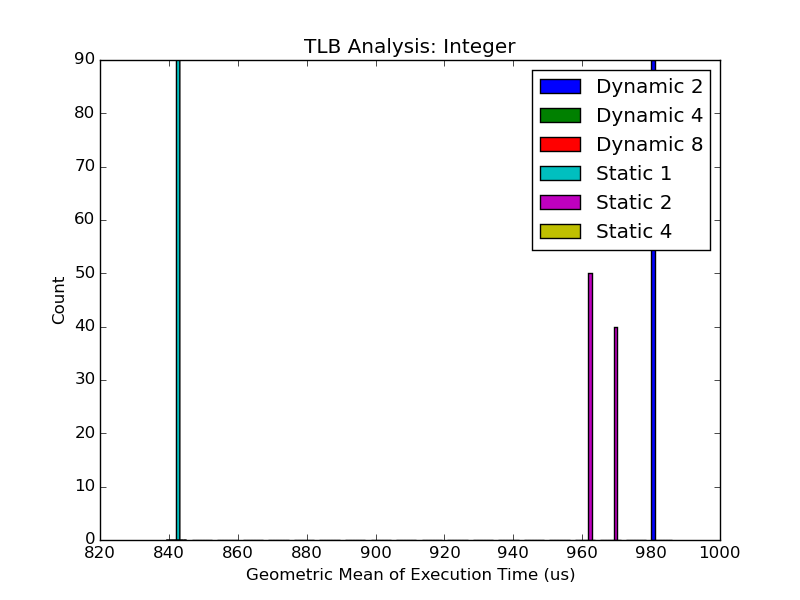
\includegraphics[width=\linewidth]{graphs/TLB/TLB_Analysis_Integer.png}
\end{minipage}\hfill
\begin{minipage}{0.5\textwidth}
\centering
 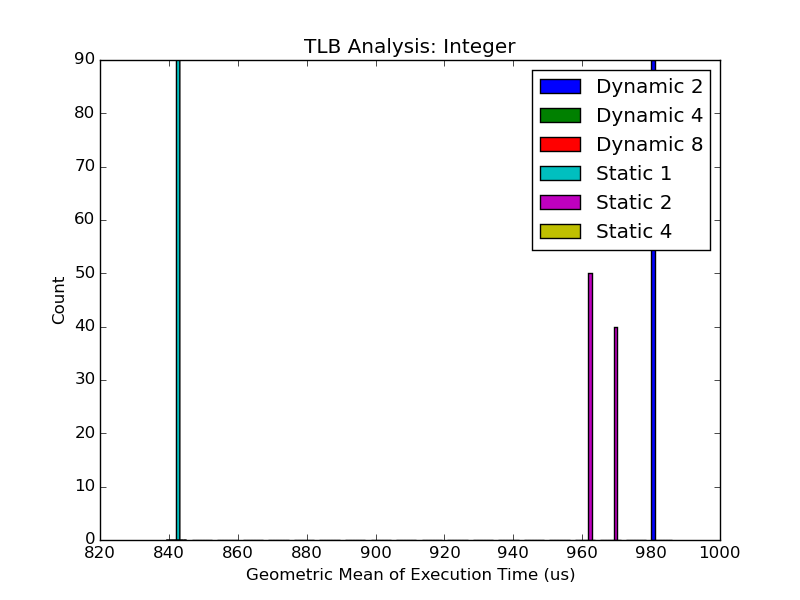
\includegraphics[width=\linewidth]{graphs/TLB/TLB_Analysis_Integer.png}
\end{minipage}

\caption{Evaluation of the TLB}
\label{fig:tlb}
\end{figure}


\section{Experiments}



\section{Conclusion}






\end{document}

